\documentclass[
  a4paper,
  english,
  DIV=16,
  11pt,
  parskip=half,
  dvipsnames,
  listof=totoc,		     % lists to toc
  index=totoc,		     % index to toc
  bibliography=totoc,	 % bibliography to toc
]{scrartcl}
\usepackage[
  pdfhighlight=/O,
  colorlinks,
  linkcolor=blue,
  urlcolor=blue,
  citecolor=black,
  filecolor=black,
  breaklinks,
  bookmarksopen,
  bookmarksopenlevel=1,
  linktocpage
]{hyperref}  % PDF support with links
\usepackage[english]{babel}
\usepackage[dvips]{graphicx}
\usepackage{eso-pic}
\usepackage[
  firstpage=true,
  scale=1,
  angle=0,
  position={current page.north},
  hshift=7.5cm, 
  vshift=-2.5cm,
  opacity=1,
  contents={%
    
\includegraphics[width=5cm,keepaspectratio]{../logos/mars_logo.png}%
  }%
]{background}
\usepackage{amsmath}
\usepackage{enumitem}
\usepackage{marvosym}
\usepackage{float}
\usepackage{microtype}
\usepackage{textcomp}
\usepackage{tikz}
\usepackage{pstricks}
\usepackage{dirtytalk}
\usepackage{xcolor}
%\usepackage[htt]{hyphenat}
%\usepackage{lmodern}
\usepackage{fontawesome}
\parindent 0pt
\bibliographystyle{alphadin}
\newcommand\todo[1]{\textcolor{red}{#1}}

\title{LaserTag}
\subtitle{An Agent-Based Simulation Game}
\author{MARS Group}
\date{\today\\Version 1.0}
\addtocontents{toc}{\protect\setcounter{tocdepth}{2}}
\setcounter{secnumdepth}{3}

\begin{document}

\maketitle
%
% ======================================================================
%
\tableofcontents
%
% ======================================================================
%
\clearpage
%
\section{Introduction}
LaserTag is an agent-based simulation game that is inspired by the real-world recreational shooting sport known as laser tag.~The game is developed with the \href{https://mars-group-haw.github.io/index.html}{Multi-Agent Research and Simulation (MARS) Framework}, which is written in \href{https://learn.microsoft.com/en-us/dotnet/csharp/}{C\#} and runs on \href{https://dotnet.microsoft.com/en-us/download}{.NET}.~Users of LaserTag can implement their own agents with customized behavioral logic by using the provided agent interface. The interface provides properties and methods which enable agent movement, agent state management, agent-agent and agent-environment interactions, and other functions.
%
\section{Game Objective} \label{sec:objective}
%
A game consists of three or four teams. Each team is made up of three agents with the same behavior logic. An agent has an energy level, which is reduced when the agent is tagged by an enemy agent. The team that depletes the energy levels of all enemy agents first wins the game.
%
% ======================================================================
%
\section{Project: Setup and Structure} \label{sec:projsetupandstruc}
%
\subsection{Project Setup} \label{ssec:projsetup}
%
Follow these steps to set up LaserTag on your machine:
%
\begin{enumerate}
  \item Install the \href{https://www.jetbrains.com/rider/}{JetBrains Rider} IDE.
  \item Clone the \href{https://github.com/MARS-Group-HAW/model-mars-laser-tag-game}{GitHub repository} that contains LaserTag.
  \item In Rider, open the directory \textbf{LaserTagBox}.
  \item If \texttt{Mars.*} dependencies are not resolved, you need to install the \href{https://www.nuget.org/packages/Mars.Life.Simulations}{MARS NuGet package}.
  \begin{enumerate}
    \item Click on the NuGet tab in the bottom bar of Rider.
    \item In the search bar, enter "Mars.Life.Simulations".
    \item Install the newest version of the NuGet package.
  \end{enumerate}
\end{enumerate}
%
\subsection{Project Structure} \label{ssec:projStruc}
%
Figure~\ref{fig:classdiag} illustrates the project structure and the properties and methods that are relevant for implementing agent behavior. For more detailed information on properties and methods, see Section~\ref{ssec:props} and Section~\ref{ssec:methods}, respectively.
%
\begin{figure}[H]
  \centering
  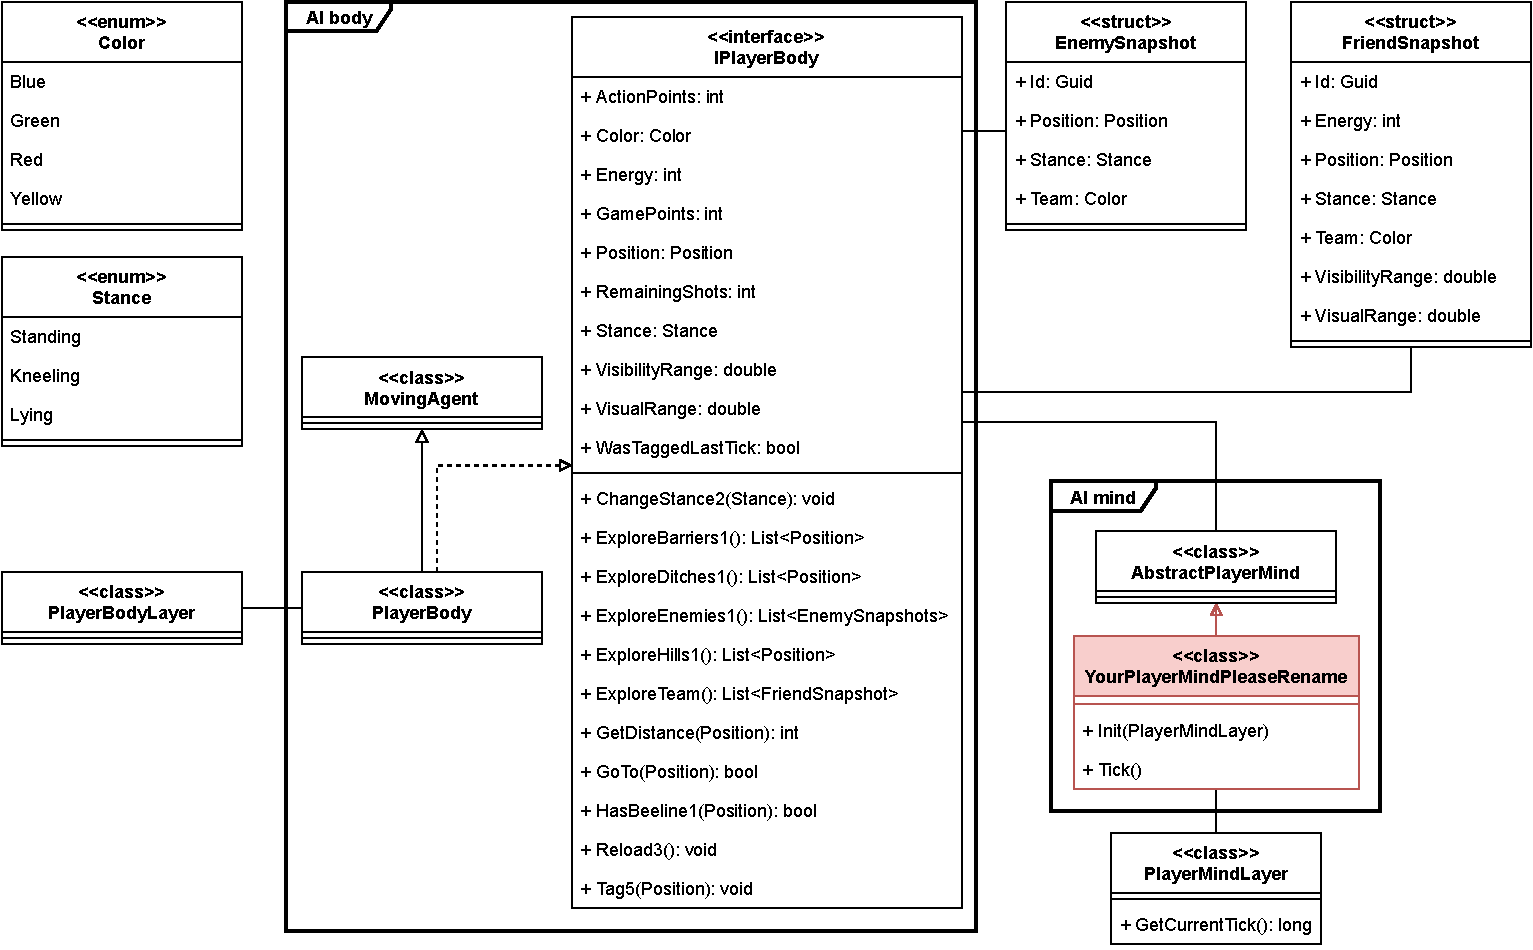
\includegraphics[width=1.0\textwidth,height=0.5\textheight,keepaspectratio]{img/LaserTagStructure.pdf}
  \caption{LaserTag class diagram}
  \label{fig:classdiag}
\end{figure}
%
The implementation of your agents occurs in a class that inherits from \texttt{AbstractPlayerMind}.~In Figure~\ref{fig:classdiag}, this is shown by the class \texttt{YourPlayerMindPleaseRename} which is labeled in red. You can rename this class and make it your own, or add other classes to the project structure that inherit from \texttt{AbstractPlayerMind}. Your agent has a reference to the \texttt{PlayerMindLayer}, from which it can obtain the current simulation tick (\texttt{GetCurrentTick()}).

In LaserTag, each agent has a mental and a physical representation -- mind and body, respectively. The mind controls the body. Through \texttt{AbstractPlayerMind}, the mind obtains a reference to the interface \texttt{IPlayerBody}.~This interface provides properties and methods that make up the agent's physical representation. The implementation of these properties and methods is found in the class \texttt{PlayerBody}. Your agent's mind can interact with the interface to guide its body and physical behavior. The class \texttt{MovingAgent} contains auxiliary properties and methods that the body requires to execute some of its functionalities.

More details regarding the enums, structs, and other parts of the model can be found in later sections of the documentation.
%
\section{Simulation: Setup and Execution} \label{sec:simSetup}
%
The game is designed to be played by three or four teams. Follow these steps to set up and play a game:
\begin{enumerate}
  \item Open the file \texttt{Program.cs}.
  \item Add your agents to the \texttt{ModelDescription} object using the provided syntax:%
  \begin{center}
    \texttt{description.AddAgent<MyAgent, PlayerMindLayer>();}
  \end{center}%
  In this example, \texttt{MyAgent} is the name of the class in which you implemented your agent.
  \item Specify the configuration file to be used for the game using the provided syntax:%
  \begin{center}
    \texttt{var file = File.ReadAllText("MyConfig.json")}.
  \end{center}%
  In this example, \texttt{MyConfig.json} is the name of the JSON file that contains the desired game configuration.
  \item Build and run the model in one of the following ways:%
  \begin{enumerate}
    \item In Rider, press the \textcolor{OliveGreen}{\Forward} Run button
    \item In a terminal, go to the directory \textbf{LaserTagBox} and enter the commands \texttt{dotnet build} and \texttt{dotnet run}.
  \end{enumerate}%
\end{enumerate}
%
The JSON file \texttt{config\_3.json} or \texttt{config\_4.json} in the directory \textbf{LaserTagBox} can be used to configure a game with three teams or four teams, respectively. Each configuration file requires resource files that need to be in the directory \textbf{Resources}:%
%
\begin{itemize}
  \item A CSV file encoding the grid-based environment
  \item A CSV file with agent parameters
\end{itemize}
%
The default environment is called \texttt{rec1\_battleground.csv}.~It encodes an environment consisting of $50\times 50$ grid cells.~The default agent initialization file for three-player and four-player games is called \texttt{player\_positions\_3.csv} and \texttt{player\_positions\_4.csv}, respectively.~Each file lists the spawn positions of the agents on the map at the beginning of the game.
%
\section{Visualization: Analyzing Game Outcomes} \label{sec:vis}
%
A Python-based tool for post-game visualization is available in the directory \textbf{Analysis}. This tool can help you analyze and improve your agents' behavior during the development process. For the tool to work, a map file (\texttt{map.csv}) is required in the directory \textbf{Resources/} and a simulation output file (\texttt{PlayerBody.csv}) is required in the directory \textbf{bin/Debug/net6.0/}.~Once these files are in place, simply double-click \texttt{vis.py} to start the visualizaton. For more detailed information, see the README file in \textbf{Analysis}.
%
% ======================================================================
%
\section{Rules} \label{sec:rules}
%
\subsection{Game Logic}
Below is a list of some of the most important parts of the game's logic:
%
\begin{itemize}
  \item If an agent's \texttt{Energy} is equal to or below 0, then the agent is taken out of the environment and does not respawn for the rest of the game. The agent's points, however, are maintained and added to the cumulative score of the team at the end of the match.
  \item An agent's \texttt{Energy} regenerates over time. At the end of each tick, an agent's \texttt{Energy} is increased by $1$.
\end{itemize}
%
\subsection{Constraints for Developers}
In order to play the game as intended, please adhere to the following rules when implementing your agents:
\begin{enumerate}
  \item Only interact with the interface \texttt{IPlayerBody} to access the agent's physical representation.
  \item When interacting with the \texttt{PlayerMindLayer}, only invoke the \texttt{GetCurrentTick()} method. Other calls to the \texttt{PlayerMindLayer} are not allowed.
  \item Your agent's constructor must be empty. %\todo{Why?}
  \item Loops that are known not to terminate after a reasonable time (example: \texttt{while(true)}) are not allowed.
  \item \texttt{PropertyDescription} tags for loading external information into your agents at runtime via an external configuration file are not allowed. The only allowed external data source is learned behavior for a learning agent.
\end{enumerate}
%
\section{Agent Properties and Methods} \label{sec:AgentDesc}
The \texttt{IPlayerBody} contains a set of properties and methods that described the agent and define its behavioral capabilities. These properties and methods can be accessed by your agents by inheriting from \texttt{AbstractAgentMind} (see Figure~\ref{fig:classdiag}).
%
\subsection{Properties} \label{ssec:props}
Below are the properties provided by the \texttt{IPlayerBody} interface that an agent's mind can access to gain information about the current state of its body.
%
\subsubsection{General properties} \label{sssec:genAttr}
\begin{itemize}
  \item \texttt{ActionPoints}: An integer that specifies the number of points the agent has to perform actions during the current tick. Each action costs a specific number of \texttt{ActionPoints} (see Section~\ref{ssec:methods} for more details). At the end of each tick, \texttt{ActionPoints} is reset to $10$.
  \item \texttt{Color}: The agent's color, indicating the team the agent belongs to.
  \item \texttt{Energy}: The agent's maximum energy level is $100$. It decreases if the agent gets tagged by an opponent. If the energy level is less than or equal to zero, the agent is removed from the simulation.
  \item \texttt{GamePoints}: the agent's score, which is increased by tagging opponents. Each tag increases the score by $10$ points. If a tag causes the tagged agent's \texttt{Energy} to be less than or equal to zero, the tagged agent loses $10$ \texttt{GamePoints} and is removed from the simulation. The tagging agent receives $10$ additional \texttt{GamePoints} as a bonus.
\end{itemize}
%
\subsubsection{Movement properties} \label{sssec:movAttr}
\begin{itemize}
  \item \texttt{Position}: Specifies the agent's current position on the map as an $(x,y)$ tuple
  \item \texttt{Stance}: An enum that specifies the agent's current stance. An agent can assume three stances:~\texttt{Standing}, \texttt{Kneeling}, and \texttt{Lying}. Each stance affects the property \texttt{VisualRange}, \texttt{VisibilityRange}, and the speed at which the agent can move.
\end{itemize}
%
\subsubsection{Exploration properties} \label{sssec:explAttr}
\begin{itemize}
  \item \texttt{VisualRange}: An integer that specifies the number of grid cells that the agent can see from its current position. The value of \texttt{VisualRange} is set based on the value of \texttt{Stance} using the following mapping:
  \begin{itemize}
    \item \texttt{Standing}$\,\to\,$10
    \item \texttt{Kneeling}$\,\to\,$8
    \item \texttt{Lying}$\,\to\,$5
  \end{itemize}
  \item \texttt{VisibilityRange}: An integer that specifies the maximum distance from which the agent can currently be seen by other agents. The value of \texttt{VisibilityRange} is set based on the value of \texttt{Stance} using the following mapping:
  \begin{itemize}
    \item \texttt{Standing}$\,\to\,$10
    \item \texttt{Kneeling}$\,\to\,$8
    \item \texttt{Lying}$\,\to\,$5
  \end{itemize}
\end{itemize}
%
\subsubsection{Tagging properties} \label{sssec:tagAttr}
\begin{itemize}
  \item \texttt{RemainingShots}: An integer that specifies the agent's currently available opportunities to tag an opponent. If the agent's \texttt{RemainingShots} is equal to zero, then a \texttt{Reload} needs to be initiated.
  \item \texttt{WasTaggedLastTick}: A boolean that specifies if the agent was tagged during the previous tick.
\end{itemize}
%
\subsection{Methods} \label{ssec:methods}
Below are the methods provided by the \texttt{IPlayerBody} interface that an agent's mind can call to guide its body. The digit at the end of the method name indicates the number of \texttt{ActionPoints} required to execute the method. Methods with no digit at the end of the name cost zero \texttt{ActionPoints}.

\faLightbulbO\: \textbf{Note:}~In general, a method call is not executed if the caller does not have enough \texttt{ActionPoints}. In this case, the method returns \texttt{false} or \texttt{null}. Please refer to individual method signatures and implementations (and the detailed descriptions below) for more information on return values of specific methods.
%
\subsubsection{Movement Methods} \label{sssec:movMeth}
\begin{itemize}
  \item \texttt{ChangeStance2(Stance)}: This method takes a \texttt{Stance} and allows the calling agent to change between three possible stances: \texttt{Standing}, \texttt{Kneeling}, and \texttt{Lying}. Stance changes affect the values of the agent's \texttt{VisualRange}, \texttt{VisibilityRange}, and movement speed (see Section~\ref{sssec:explAttr}). This method has no return value.
  \item \texttt{GoTo(Position) :~bool}: This is the main method used for pathfinding, movement, and path readjustment. When an agent invokes the method, the method devises a path from the agent's current position to the given \texttt{Position}. Each subsequent invocation of \texttt{GoTo(Position)} with the same destination will, if possible, move the agent one step closer to the destination until the destination is reached.
  
  In order for the agent to change its path before reaching its current destination, \texttt{GoTo(Position)} must be called with a different destination. For example, if the agent is currently moving towards the \texttt{Position} (a, b), this movement process can be interrupted and replaced by a new movement process by calling \texttt{goto((c, d))}, where \texttt{c != a} or \texttt{d != b}.
  
  The method returns \texttt{true} if a move was made and \texttt{false} if, for any reason, a move was not made.
  
  \faLightbulbO\: \textbf{Note:}~If \texttt{GoTo(Position)} is called with a destination that refers to a grid cell that is inaccessible (because there is a \texttt{Barrier} on it or because it lies outside of the environment), then no path is calculated and no movement is initiated.
  
  For more information on \texttt{GoTo(Position)}, see Section~\ref{sssec:movement}.
\end{itemize}
%
\subsubsection{Exploration methods} \label{sssec:explMeth}
\begin{itemize}
  \item \texttt{ExploreBarriers1() :~List<Position>}: Returns a (potentially empty) list of positions of \texttt{Barrier} objects that are in the caller's \texttt{VisualRange} and which the caller can see (\texttt{HasBeeline == true}).
  
  \faLightbulbO\: \textbf{Note:} Returns \texttt{null} if the caller does not have enough \texttt{ActionPoints}.
  %
  \item \texttt{ExploreDitches1() :~List<Position>}: Returns a list of positions of \texttt{Ditch} objects that are in the caller's \texttt{VisualRange} and which the caller can see (\texttt{HasBeeline == true}).
  
  \faLightbulbO\: \textbf{Note:} Returns \texttt{null} if the caller does not have enough \texttt{ActionPoints}.
  %
  \item \texttt{ExploreHills1() :~List<Position>}: Returns a list of positions of \texttt{Hill} objects that are in the caller's \texttt{VisualRange} and which the caller can see (\texttt{HasBeeline == true}).
  
  \faLightbulbO\: \textbf{Note:} Returns \texttt{null} if the caller does not have enough \texttt{ActionPoints}.
  %
  \item \texttt{ExploreEnemies1() :~List<EnemySnapshot>}: Performs an exploration of opponents in the caller's \texttt{VisualRange} and which the caller can see (\texttt{HasBeeline == true}). Returns a list of \texttt{EnemySnapshot} structs, offering limited information about the identified opponents.
  
  \faLightbulbO\: \textbf{Note:} Returns \texttt{null} if the caller does not have enough \texttt{ActionPoints}.
  %
  \item \texttt{ExploreTeam() :~List<IPlayerBody>}: Returns a list of \texttt{FriendSnapshot} structs, offering limited information about the caller's team members.
  %
  \item \texttt{GetDistance(Position) :~int}: Returns the shortest distance (measured in the the number of grid cells) from the caller's current position to the specified \texttt{Position}. In order for the distance to be calculable, the grid cell specified by \texttt{Position} must be visible (based on \texttt{HasBeeline1(Position)}). If the distance to the grid cell specified by \texttt{Position} is not calculable, the method returns \texttt{-1}.
  %
  \item \texttt{HasBeeline1(Position) :~bool}: This method may be called by an agent to check if the line of sight between its current position and the grid cell denoted by \texttt{Position} is free from vision-blocking obstacles (i.e., \texttt{Barrier} or \texttt{Hill} objects). If it is, the method returns \texttt{true}. If it is not (or if the caller does not have enough \texttt{ActionPoints}), the method returns \texttt{false}.

  \faLightbulbO\: \textbf{Note:} Returns \texttt{false} if the caller does not have enough \texttt{ActionPoints}.
\end{itemize}
%
\subsubsection{Tagging methods} \label{sssec:tagMeth}
\begin{itemize}
  \item \texttt{Tag5(Position)}: This method takes a \texttt{Position} and prompts the calling agent to fire a shot onto the grid cell encoded by the position. If an enemy agent is currently located at that position, then that agent is tagged.
  
  Tagging is implemented as a probability-based process that is influenced by both agents' \texttt{Stance} and current positions (ground, \texttt{Hill}, or \texttt{Ditch}). For example, an agent in the \texttt{Lying} stance has higher accuracy but shorter \texttt{VisualRange}. If an agent is tagged, its \texttt{Energy} is decreased by $10$ and the property \texttt{WasTaggedLastTick} is set to \texttt{true}. The tagging agent's \texttt{GamePoints} is increased by $10$.

  \faLightbulbO\: \textbf{Note:} Returns \texttt{false} if the caller does not have enough \texttt{ActionPoints}.
  
  For more information on tagging, see Section \ref{sssec:tagging}.
  %
  \item \texttt{Reload3()}: Reloads the caller's tag gun. This is necessary when \texttt{RemainingShots == 0} so that the agent can continue tagging enemies. A successful call to \texttt{Reload3()} refills the calling agent's \texttt{RemainingShots} to $5$. This method does not return anything.

\end{itemize}
%
% ======================================================================
%
\section{Model Description} \label{sec:modelDesc}
The model's main components are the environment and the properties and methods that serve as an interface for the agents to shape their behavior and decision-making and interact with their environment and with each other.
%
\subsection{The Environment} \label{ssec:env}
The default environment is a $50\times 50$ grid layer. In order to effectively simulate the indoor nature of real-world laser tag, the environment is fenced in. To add texture and complexity to the environment and to allow agents to interact with it meaningfully, maps may feature structures (barriers, rooms, hills, and ditches).

Figure~\ref{fig:envEx} shows a bird's eye view of an example of a square-shaped map at the start of the simulation. The following sections describe each of the spots. For more information on spots, see Sections \ref{sssec:vision}, \ref{sssec:tagging}, and \ref{sssec:spot}.
%
\begin{figure}[H]
  \centering
  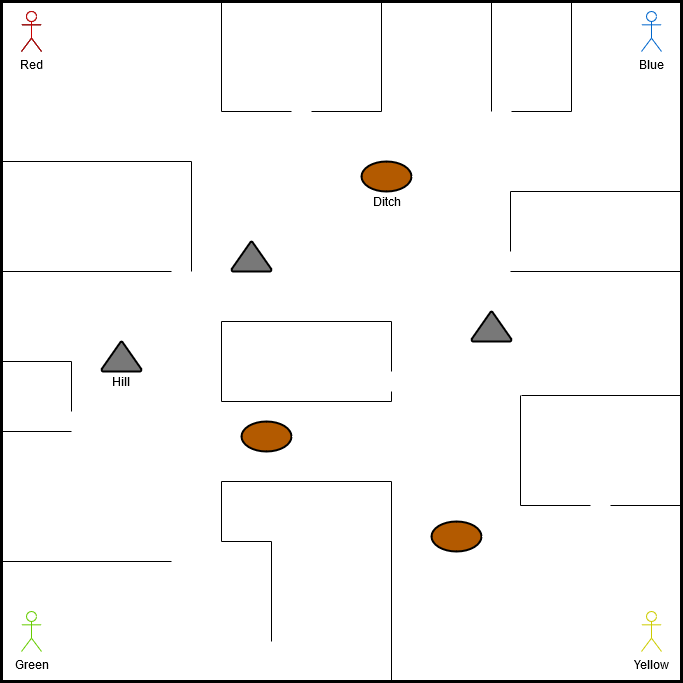
\includegraphics[width=0.5\textwidth, height=0.5\textheight,keepaspectratio]{img/ExampleGameWorldAtSimStart.png}
  \caption{Example of square-shaped map environment at simulation start (not drawn to scale)}
  \label{fig:envEx}
\end{figure}
%
\subsubsection{Structures} \label{sssec:struc}
There are a few structural elements in the environment that agents can interact with by calling one of the \texttt{Explore*} methods (except \texttt{ExploreTeam} and \texttt{ExploreEnemies1}). Figure~\ref*{fig:structures} shows the inheritance hierarchy of the structures. Each exploration costs one \texttt{ActionPoint}.
%
\begin{figure}[H]
    \centering
    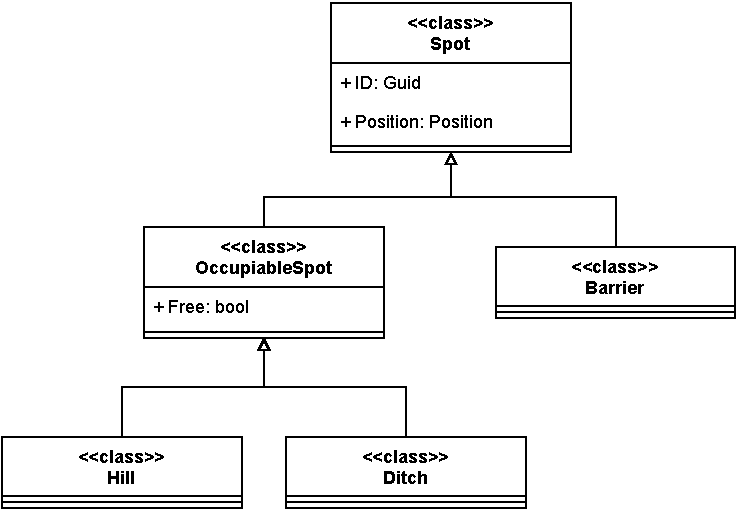
\includegraphics[width=0.5\textwidth, height=0.5\textheight,keepaspectratio]{img/lasertag-env-comps.pdf}
    \caption{Structures}
    \label{fig:structures}
\end{figure}
%
\paragraph{Barrier} \label{par:barrierDesc}
A \texttt{Barrier} is a structure that cannot be occupied, that acts as an impermeable obstacle to agents, and that disrupts an agent's vision. \texttt{Barrier} instances can be explored by calling \texttt{ExploreBarrier1}.
%
\paragraph{Hill} \label{par:hillDesc}
A \texttt{Hill} is a structure that can be occupied. While an agent occupies a \texttt{Hill}, the agent's \texttt{VisualRange} and \texttt{Visibility} are increased. The probability of the agent getting tagged also increases. Occpying a \texttt{Hill} might be a useful team tactic: An agent on a \texttt{Hill} can spot for another agent who is on the ground. \texttt{Hill} instances can be explored by calling \texttt{ExploreHill1}.
%
\paragraph{Ditch} \label{par:ditchDesc}
A \texttt{Ditch} is a structure that can be occupied. While an agent occupies a \texttt{Ditch}, the agent's \texttt{VisualRange} and \texttt{Visibility} are decreased. The probability of the agent getting tagged also decreases. Occpying a \texttt{Ditch} might be a useful for ambushing enemies. \texttt{Ditch} instances can be explored by calling \texttt{ExploreDitch1}.
%
\paragraph{Room} \label{par:roomDesc}
A room is a section of the grid layer that is enclosed by barriers, leaving only one or more small gaps to enter and exit the enclosed section.
%
\subsubsection{Designing your own maps}
%
You can design your own LaserTag environments. To do so, create a CSV file and follow these guidelines:
%
\begin{itemize}
  \item The shape of your map must be rectancular ($n \times m$) or square ($n \times n$).
  \item Use a semicolon (\texttt{;}) as a separator.
  \item Use the following encoding for LaserTag structures (see Section~\ref{sssec:struc} for more details):
  \begin{itemize}
    \item 0$\,\to\,$empty cell
    \item 1$\,\to\,$\texttt{Barrier}
    \item 2$\,\to\,$\texttt{Hill}
    \item 3$\,\to\,$\texttt{Ditch}
  \end{itemize}
\end{itemize}
%
For reference and examples, see the default maps in the directory \texttt{LaserTagBox/Resources/}.
%
\subsection{Game Mechanics} \label{ssec:gameMechs}
%
This section outlines some of the built-in logic, mechanisms, and rules of LaserTag to help you devise intelligent and feasible strategies for your agents.
%
\subsubsection{Vision} \label{sssec:vision}
The game features a vision system that depends on a number of variables and circumstances. The following example aims to illustrate the process. Agent X calls \texttt{ExploreEnemies1()} and hopes to see agent Y. X's ability to see Y may be influenced by each of the following conditions:
%
\begin{enumerate}
  \item the relation between \texttt{distance(X, Y)} and X's \texttt{VisualRange}.
  \item the relation between \texttt{Distance(X, Y)} and Y's \texttt{VisibilityRange}.
  \item whether X or Y is currently located on a \texttt{Hill}.
  \item whether X or Y is currently located in a \texttt{Ditch}.
  \item whether the line of sight between X and Y is obstructed by a barrier or hill.
\end{enumerate}
%
Let us examine each condition in turn:
%
\begin{enumerate}
  \item If the distance between X and Y is less than or equal to X's \texttt{VisualRange}, then X may be able to see Y.
  \item If the distance between X and Y is less than or equal to Y's \texttt{VisibilityRange}, then X may be able to see Y. Y's \texttt{VisibilityRange} is irrelevant for when X stands either on a \texttt{Hill} or in a \texttt{Ditch}.
  \item A barrier or \texttt{Hill} can block an agent's line of sight. If there is nothing blocking X's line of sight to Y, then X may be able to see Y. For more information on line-of-sight computation, feel free to check out \href{http://tech-algorithm.com/articles/drawing-line-using-bresenham-algorithm/}{Bresenham's Line Algorithm} which is implemented in LaserTag to determine if any of the grid cells along the line of sight between two agents holds an vision-blocking object (a barrier or \texttt{Hill}).
  \item If X is located on a \texttt{Hill}, then his \texttt{VisualRange} is increased, making it possible for him to see Y from a farther distance. Likewise, if Y is located on a hill, then his \texttt{VisibilityRange} is increased, making it easier for X to see him.
  \item If X is located in a \texttt{Ditch}, then his \texttt{VisualRange} is decreased, which requires Y to be closer to X in order for X to be able to see Y. Likewise, if Y is located in a \texttt{Ditch}, then his \texttt{VisibilityRange} is decreased, requiring X to be closer to Y in order for X to be able to see Y.
\end{enumerate}
%
Conditions 1, 2, and 3 must be met in order for X to be able to see Y. Conditions 4 and 5 merely describe how standing on a \texttt{Hill} or in a \texttt{Ditch} might affect the vision process.
%
\subsubsection{Movement} \label{sssec:movement}
Agents move along the grid via a modified version of the \href{http://idm-lab.org/bib/abstracts/papers/aaai02b.pdf}{D* Lite Algorithm}. The algorithm computes an initial (usually close-to-optimal or optimal) route from an agent's current position to the desired destination. Once the route has been calculated, the algorithm guides the agent towards the goal at a rate dependent on the agent's \texttt{Stance} and movement capabilities. The algorithm performs route adjustments and recalculations only if an obstacle intersects the agent's path that was not present during the initial route computation. This makes the algorithm highly efficient and perform at a better time complexity than more common path-finding algorithms such as A*.
%
\subsubsection{Tagging} \label{sssec:tagging}
Tagging is the core game mechanic that drives LaserTag. In an attempt to simulate real-world tag-and-get-tagged interactions between laser tag players, the method \texttt{Tag5(Position)} relies on probability and randomization to create a balance between successful and unsuccessful tag attempts. If agent X attempts to tag agent Y, the outcome depends on the following factors:
%
\begin{enumerate}
  \item X's \texttt{Stance}
  \item Y's \texttt{Stance}
  \item whether Y is currently positioned on a regular grid cell, a hill, or a ditch
  \item a dose of luck
\end{enumerate}
%
Let us examine each factor in turn:
%
\begin{enumerate}
  \item If X's \texttt{Stance == Lying}, then he is most likely to tag Y. If X's \texttt{Stance == Standing}, then he is least likely to tag Y.
  \item If Y's \texttt{Stance == Standing}, then X is most likely to tag him. If Y's \texttt{Stance == Lying}, then X is least likely to tag him.
  \item If Y is located on a \texttt{Hill}, then his \texttt{Stance} cannot lower the likelihood of him being tagged. This is because being on a \texttt{Hill} leads to more exposure than being on the ground or in a \texttt{Ditch}. Conversely, if Y is located in a \texttt{Ditch}, then his \texttt{Stance} does not increase his likelihood of being tagged. This is because a being in a \texttt{Ditch} provides increased cover regardless of the agent's \texttt{Stance}.
  \item Even if factors 1-3 are in Y's favor, there is still a chance that X tags Y. On the other hand, even if factors 1-3 are in X's favor, there is still a chance that he might miss Y and not tag him. This is due to the element of randomization added to the tagging mechanism.
\end{enumerate}
%
\subsubsection{Spots} \label{sssec:spot}
The environment features \texttt{Hill}, \texttt{Ditch}, and \texttt{Barrier} objects for agents to interact with and, under certain circumstances, gain an advantage over their opponents. A \texttt{Barrier} object cannot be occupied. A \texttt{Hill} or \texttt{Ditch} can be occupied by only one agent at a time. Being on a \texttt{Hill} increases an agent's \texttt{VisualRange} and \texttt{VisibilityRange} by five each. Being in a \texttt{Ditch} lowers an agent's \texttt{VisualRange} and  \texttt{VisibilityRange} by three each. See Sections \ref{sssec:vision}, \ref{sssec:tagging}, \ref{par:hillDesc}, and \ref{par:ditchDesc} for more information.

\end{document}
